%% ##############################################################################################
%%
%% Copyright 2012 CNRS, INPT
%%  
%% This file is part of qr_mumps.
%%  
%% qr_mumps is free software: you can redistribute it and/or modify
%% it under the terms of the GNU Lesser General Public License as 
%% published by the Free Software Foundation, either version 3 of 
%% the License, or (at your option) any later version.
%%  
%% qr_mumps is distributed in the hope that it will be useful,
%% but WITHOUT ANY WARRANTY; without even the implied warranty of
%% MERCHANTABILITY or FITNESS FOR A PARTICULAR PURPOSE.  See the
%% GNU Lesser General Public License for more details.
%%  
%% You can find a copy of the GNU Lesser General Public License
%% in the qr_mumps/doc directory.
%%
%% ##############################################################################################

%% 
%% $Date: 2015-10-27 22:41:03 +0100 (mar., 27 oct. 2015) $
%% $Author: abuttari $
%% $Version: 1.1$
%% $Revision: 1980 $
%%

\documentclass[11pt]{article}
\usepackage{qrm}

\begin{document}

%% ##############################################################################################
%%
%% Copyright 2012 CNRS, INPT
%%  
%% This file is part of qr_mumps.
%%  
%% qr_mumps is free software: you can redistribute it and/or modify
%% it under the terms of the GNU Lesser General Public License as 
%% published by the Free Software Foundation, either version 3 of 
%% the License, or (at your option) any later version.
%%  
%% qr_mumps is distributed in the hope that it will be useful,
%% but WITHOUT ANY WARRANTY; without even the implied warranty of
%% MERCHANTABILITY or FITNESS FOR A PARTICULAR PURPOSE.  See the
%% GNU Lesser General Public License for more details.
%%  
%% You can find a copy of the GNU Lesser General Public License
%% in the qr_mumps/doc directory.
%%
%% ##############################################################################################

%% 
%% $Date: 2015-10-27 22:41:03 +0100 (mar., 27 oct. 2015) $
%% $Author: abuttari $
%% $Version: 1.1$
%% $Revision: 1980 $
%%

\begin{adjustwidth}{-0em}{-0em}
\thispagestyle{empty}


\vspace{10cm}
\vspace*{\stretch{1}}

{\noindent\hfill 
\includegraphics[width=0.9\linewidth]{figures/qrqr_cover.pdf}}

\noindent\rule{\linewidth}{5pt}\\[2.5ex]

\vspace{1cm}

\hspace{\stretch{1}}{\Large Users guide}
% \hspace{\stretch{1}}{\Large Alfredo Buttari}

% \hspace{\stretch{1}}{\large CNRS-IRIT}

% \hspace{\stretch{1}}{\large 19/01/2012}

\vspace*{\stretch{2}}

\end{adjustwidth}
%%% Local Variables: 
%%% mode: latex
%%% TeX-master: "qrm_ug"
%%% End: 


\newpage

\tableofcontents
\newpage

\section{Introduction}
\label{sec:intro}

\qrm is a software package for the solution of sparse, linear systems
on multicore computers. It implements a direct solution method based
on the $QR$ factorization of the input matrix. Therefore, it is suited
to solving sparse {\bf least-squares} problems $\min_x\|Ax-b\|_2$ and
to computing the {\bf minimum-norm} solution of sparse,
underdetermined problems. It can obviously be used for solving square
problems in which case the stability provided by the use of orthogonal
transformations comes at the cost of a higher operation count with
respect to solvers based on, e.g., the $LU$ factorization. \qrm
supports {\bf real and complex}, {\bf single or double} precision
arithmetic.

As in all the sparse, direct solvers, the solution is achieved in
three distinct phases:
\begin{description}
\item[Analysis]: in this phase an analysis of the structural properties
  of the input matrix is performed in preparation for the numerical
  factorization phase. This includes computing a column permutation
  which reduces the amount of {\it fill-in} coefficients (i.e.,
  nonzeroes introduced by the factorization). This step does not
  perform any floating-point operation and is, thus, commonly mush
  faster than the factorization and solve (depending on the number of
  right-hand sides) phases.
\item[Factorization]: at this step, the actual $QR$ factorization is
  computed. This step is the most computationally intense and,
  therefore, the most time consuming.
\item[Solution]: once the factorization is done, the factors can be used
  to compute the solution of the problem through two operations:
  \begin{description}
  \item[Solve] : this operation computed the solution of the
    triangular system $Rx=b$ or $R^Tx=b$;
  \item[Apply] : this operation applies the $Q$ orthogonal matrix to a
    vector, i.e., $y = Qx$ or $y = Q^Tx$.
  \end{description}
\end{description}

These three steps have to be done in order but each of them can be
performed multiple times. If, for example, the problem has to be
solved against multiple right-hand sides (not all available at once),
the analysis and factorization can be done only once while the
solution is repeated for each right-hand side. By the same token, if
the coefficients of a matrix are updated but not its structure, the
analysis can be performed only once for multiple factorization and
solution steps.

\qrm is built upon the large knowledge base and know-how developed by
the members of the MUMPS\footnote{\url{http://mumps.enseeiht.fr}}
project. However, \qrm does not share any code with the MUMPS package
and it is a completely independent software. \qrm is developed and
maintained in a collaborative effort by the IRIT-CERFACS joint
laboratory in Toulouse, the ROMA team at ENS-Lyon and the LaBRI
laboratory in Bordeaux, France.



\section{Algorithm}
\label{sec:algo}

\qrm is based on the multifrontal factorization method. This method
was first introduced by Duff and Reid~\cite{dure:83} as a method for
the factorization of sparse, symmetric linear systems and, since then,
has been the object of numerous studies and the method of choice for
several, high-performance, software packages such as
MUMPS~\cite{adkl:00} and UMFPACK~\cite{davis:04}. At the heart of this
method is the concept of an {\it elimination tree}, extensively
studied and formalized later by Liu~\cite{liu:90}. This tree graph
describes the dependencies among computational tasks in the
multifrontal factorization. The multifrontal method can be adapted to
the $QR$ factorization of a sparse matrix thanks to the fact that the
$R$ factor of a matrix $A$ and the Cholesky factor of the normal
equation matrix $A^TA$ share the same structure under the hypothesis
that the matrix $A$ is {\it Strong Hall} (for a definition of this
property see, for example,~\cite{bjor:96}). Based on this equivalence,
the elimination tree for the $QR$ factorization of $A$ is the same as
that for the Cholesky factorization of $A^TA$. In the case where the
Strong Hall property does not hold, the elimination tree related to
the Cholesky factorization of $A^TA$ can still be used although the
resulting $QR$ factorization will perform more computations and
consume more memory than what is really needed; alternatively, the
matrix $A$ can be permuted to a Block Triangular Form (BTF) where all
the diagonal blocks are Strong Hall.

In a basic multifrontal method, the elimination tree has $n$ nodes,
where $n$ is the number of columns in the input matrix $A$, each node
representing one pivotal step of the $QR$ factorization of $A$. Every
node of the tree is associated with a dense matrix, known as {\it
  frontal matrix} that contains all the coefficients affected by the
elimination of the corresponding pivot. The whole $QR$ factorization
consists in a bottom-up traversal of the tree where, at each node, two
operations are performed:

\begin{itemize}
\item {\bf assembly}: a set of rows from the original matrix
  is assembled together with data produced by the processing of child
  nodes to form the frontal matrix;
\item {\bf factorization}: one Householder reflector is computed and
  applied to the whole frontal matrix in order to annihilate all the
  subdiagonal elements in the first column. This step produces one row
  of the $R$ factor of the original matrix and a complement which
  corresponds to the data that will be later assembled into the parent
  node (commonly referred to as a {\it contribution block}). The $Q$
  factor is defined implicitly by means of the Householder vectors
  computed on each front; the matrix that stores the coefficients of
  the computed Householder vectors, will be referred to as the $H$
  matrix from now on.
\end{itemize}

\begin{figure}[ht]
\begin{minipage}[b]{0.5\textwidth}
\centering
  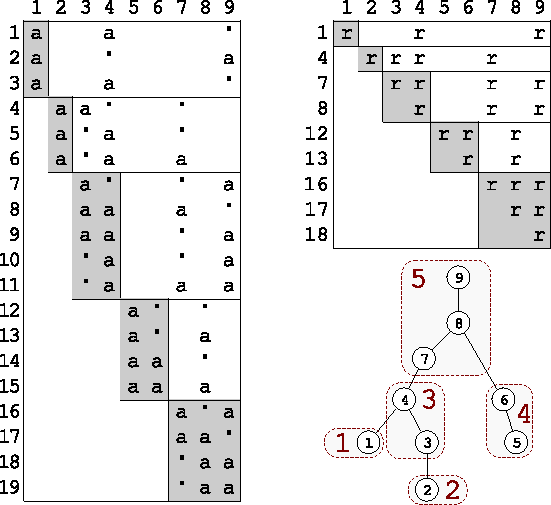
\includegraphics[width=\textwidth]{figures/mfront}
\end{minipage}
\hspace{0.5cm}
\begin{minipage}[b]{0.5\textwidth}
\centering
  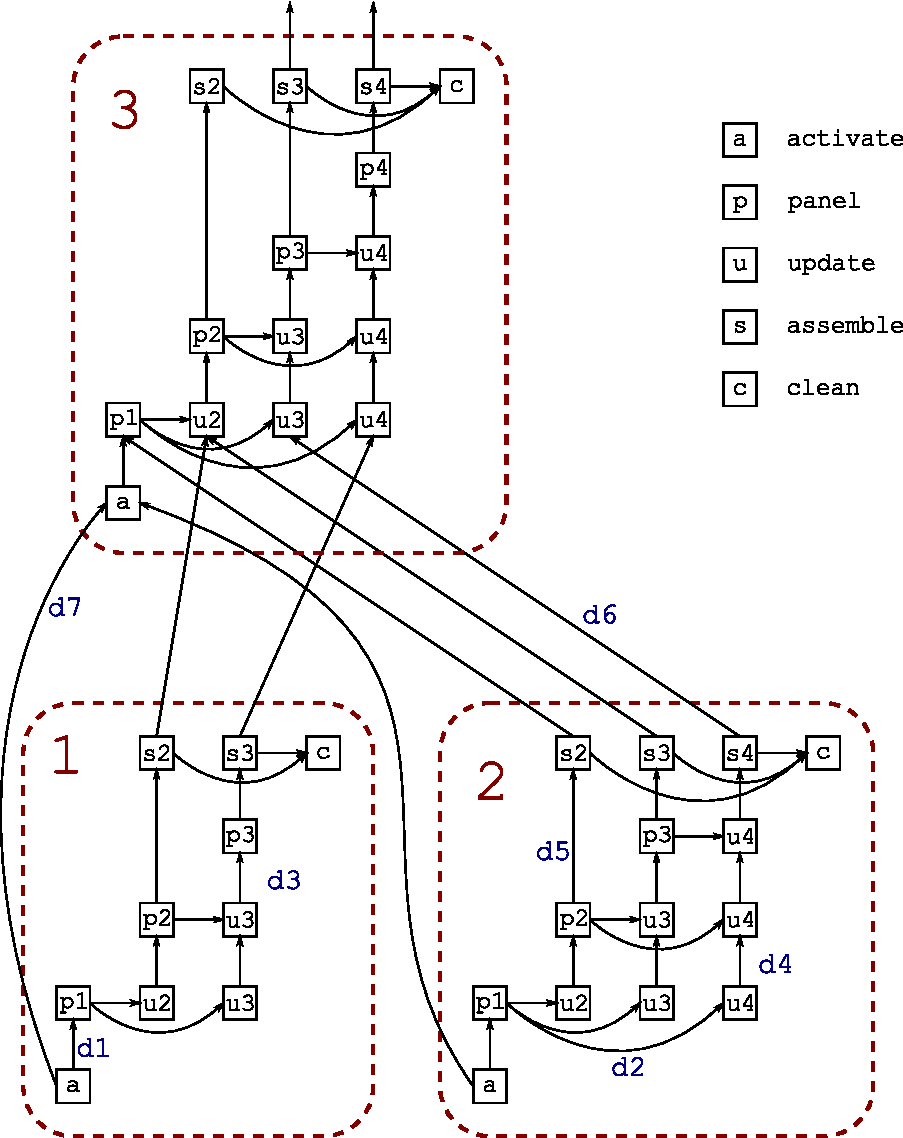
\includegraphics[width=0.8\textwidth]{figures/dag}
\end{minipage}
\caption{\label{fig:qrmfront}{\it (left)} Example of multifrontal $QR$
  factorization. The dots denote the fill-in coefficients. {\it
    (right)} The DAG associated with supernodes 1, 2 and 3 for a
  block-column size of one.}
\end{figure}


In practical implementations of the multifrontal $QR$ factorization,
and in \qrm, nodes of the elimination tree are amalgamated to form
{\it super nodes}. The amalgamated pivots correspond to rows of $R$
that have the same structure and can be eliminated at once within the
same frontal matrix without producing any additional fill-in in the
$R$ factor. The elimination of amalgamated pivots and the consequent
update of the trailing frontal submatrix can thus be performed by
means of efficient Level-3 BLAS routines. Moreover, amalgamation
reduces the number of assembly operations increasing the
computations-to-communications ratio which results in better
performance. The amalgamated elimination tree is also commonly
referred to as {\it assembly tree}. Figure~\ref{fig:qrmfront} {\it
  (left)} shows a sparse matrix along with the assembly tree and the
resulting $R$ factor.

Parallelism is exploited, in \qrm, thorough a fine-grained
decomposition of the frontal matrices into block-columns. As
illustrated in Figure~\ref{fig:qrmfront} {\it (right)}, this allows
representing the whole matrix factorization as DAG (Directed Acyclic
Graph) where nodes represent sequential tasks, i.e. the execution of
one elementary operation on a block-column, and edges the dependencies
among them. 

The tasks in the DAG are then scheduled dynamically according to a
data-flow parallel execution model. This approach delivers high
flexibility and concurrence which result in high performance on
modern, multicore computers.  

The method used in \qrm is described in full details
in~\cite{butt:11}. 

\section{Features}
\subsection{Parallelism}
\label{sec:parallelism}
\qrm is a parallel, multithreaded software based on the OpenMP
standard. Therefore, it will run on multicore or, more generally,
shared memory multiprocessor computers. \qrm does not run on
distributed memory (e.g. clusters) parallel computers. As described in
Section~\ref{sec:algo}, parallelism is achieved through a
decomposition of the workload into fine-grained computational tasks
which basically correspond to the execution of a BLAS or LAPACK
operation on a block-column. It is strongly recommended to use
sequential BLAS and LAPACK libraries and let \qrm have full control of
the parallelism. Equivalently, you can link to a multithreaded BLAS or
LAPACK making sure the number of threads used by these libraries is
equal to one when \qrm routines are called. For example, for OpenMP
based BLAS libraries, such as Intel MKL, executing \texttt{call
  omp\_set\_num\_threads(1)} right before a \qrm routine will do.

The number of threads used by \qrm can be controlled in two different
ways:
\begin{enumerate}
\item by setting \texttt{QRM\_NUM\_THREADS} environment variable to the desired
  number of threads. In this case the number of threads will be the
  same throughout the execution of your program/application;
\item through the \texttt{qrm\_set} (see Section~\ref{sec:set}
  and~\ref{sec:cntl}). This allows a finer control over the
  parallelism; for example, a different number of threads can be used
  in two consecutive calls to the factorization phase.
\end{enumerate}

The \texttt{qrm\_set} routine has higher priority than the
\texttt{QRM\_NUM\_THREADS} environment variable. 

The granularity of the tasks is controlled by the \texttt{qrm\_nb\_}
parameter (see Section~\ref{sec:cntl}) which is a blocking factor for
partitioning internal data. Smaller values mean more parallelism;
however, because this blocking factor is an upper-bound for the
granularity of operations (or, more precisely for the granularity of
calls to BLAS and LAPACK routines), it is recommended to choose
reasonably large values in order to achieve high efficiency. 
Experimental results show that 120 gives a good compromise between
concurrence and efficiency of elementary operations over a wide range of
modern, multicore architectures (such as Intel, AMD or IBM processors).


\subsection{Singletons detection}
\label{sec:singleton}
The analysis phase in a $QR$ multifrontal solver heavily relies on the
assumption that the structure of the $R$ factor of $A$ is the same as
that of the Cholesky factor of $A^TA$. However, this assumption does
not hold when the $A$ matrix is not {\it strong Hall}, in which case the
analysis may largely overestimate the fill-in. This problem can be
addressed by permuting the input matrix to a Block Triangular Form
(BTF): this will not only reduce the cost of the factorization phase
because only the diagonal block must be factorized but, since these
are strong Hall, will also make the analysis perfectly accurate (for
further details please refer to Puglisi et al.~\cite{pugl:93}). \qrm
does not directly provide the possibility to permute the matrix
into BTF (it is obviously possible for the user to do it and then
invoke \qrm separately on each diagonal block); instead it provides a
feature called {\it singleton detection} introduced by Tim Davis in
the SPQR~\cite{Davis:2011:A9S:2049662.2049670} package. This feature
consists in permuting the input matrix as
\begin{displaymath}
  PAQ = \left[
    \begin{array}{cc}
      R_{11} & R_{12} \\
      0      & \tilde{A}_{22}\\
    \end{array}\right]
\end{displaymath}
where $R_{11}$ is upper triangular. In this case on the
$\tilde{A}_{22}$ submatrix will be factorized. It has to be noted that
the singleton detection does not guarantee that the $\tilde{A}_{22}$
submatrix is strong Hall although it commonly makes the problem much
more tractable.

The singleton detection feature can be turned on or off through the
\texttt{qrm\_set} routine (see Section~\ref{sec:cntl}).


\subsection{Orderings}
The cost of a sparse matrix factorization (both in terms of floating
point operations and memory footprint) heavily depends on the amount
of fill-in. In the case of a $QR$ factorization, this can be reduced
by conveniently permuting the columns of the input matrix. \qrm
supports several permutation methods (commonly called pivot ordering
methods) through third party software packages, namely
COLAMD~\cite{Davis:2004:CAM:1024074.1024079}, SCOTCH~\cite{pelle:07}
and Metis~\cite{Karypis:1998:FHQ:305219.305248}. It is also possible
for the user to provide his own column permutation of choice. Methods
based on nested dissection (i.e., those in SCOTCH and Metis) commonly
provide better results and are, therefore, highly recommended
especially on larger matrices. The ordering method can be chosen using
the \texttt{qrm\_set} routine (see Section~\ref{sec:cntl}).


% \section{Installation and usage}

\newpage
\section{API}
\qrm is developed in the Fortran 2003 language\footnote{or, better,
  Fortran 95 plus a minor subset of the Fortran 2003 features.} but
includes a C interface developed through the Fortran 2003
\texttt{iso\_c\_binding} feature. All the \qrm features are available
from both interfaces although the Fortran one takes full advantage of
the language features, such as the interface overloading, that are
not available in C.  The naming convention used in \qrm groups all the
routine or data type names into two families depending on whether they
depend on the arithmetic or not. Typed names always begin by
\texttt{\_qrm\_} where the first underscore \_ becomes \texttt{d},
\texttt{s}, \texttt{z}, \texttt{c} for real double, real single,
complex double or complex single arithmetic, respectively. Untyped
names, instead, simply begin by \texttt{qrm\_}. Note that thanks to
interface overloading in Fortran all the typed interfaces of a routine
can be conveniently grouped into a single untyped one; this is
described in details in Section~\ref{sec:iover}.  All the interfaces
described in the remainder of this section are for the real, single
precision case. The interfaces for real double, complex single and
complex double can be obtained by replacing \texttt{sqrm} with
\texttt{dqrm}, \texttt{cqrm} and \texttt{zqrm}, respectively and
\texttt{real} with \texttt{real(kind(1.d0))}, \texttt{complex},
\texttt{complex(kind(1.d0))}, respectively. All the routines that take
vectors as input (e.g., \texttt{\_qrm\_apply}) can be called with
either one vector (i.e. a rank-1 Fortran array \texttt{x(:)}) or
multiple ones (i.e., a rank-2 Fortran array \texttt{x(:,:)}) through
the same interface thanks to interface overloading. This is not
possible for the C interface, in which case an extra argument is
present in order to specify the number of vectors which are expected
to be stored in column-major (i.e., Fortran style) format.

In this section only the Fortran API is presented. For each Fortran
name (either of a routine or of a data type) the corresponding C name
is obtained by adding the \texttt{\_c} suffix. The number, type and
order of arguments in the C routines is the same except for those
routines that take dense vectors in which case, the C interface needs
an extra argument specifying the number of vectors passed trough the
same pointer. The user can refer to the code examples and to the
\texttt{\_qrm\_mumps.h} file for the full details of the C interface.


% \renewcommand{\labelitemi}{-}

\subsection{Data types}
\subsubsection{\texttt{\_qrm\_spmat\_type}}
This data type is used to define a problem and all the information
needed to process it. Specifically it contains the problem matrix, the
parameters used to control the behavior of the \qrm operations done on
it and the statistics collected by \qrm during the execution of these
operations.

%\lst{listings/qrm_spmat_type.f90}{listings/qrm_spmat_type_c.c}
\lsts{listings/qrm_spmat_type.f90}

\begin{itemize}
\item Matrix data: matrices can be stored in the \texttt{COO} (or
  coordinate) format through the \texttt{irn}, \texttt{jcn} and
  \texttt{val} fields containing the row indices, column indices and
  values, respectively and the \texttt{m}, \texttt{n} and \texttt{nz}
  containing the number of rows, columns and nonzeroes,
  respectively. \qrm uses a Fortran-style 1-based numbering and thus
  all row indices are expected to be between 1 and \texttt{m} and all
  the column indices between 1 and \texttt{n}. Duplicate entries are
  summed during the factorization, out-of-bound entries are ignored.
\item \texttt{cperm\_in}: this array can be used to provide a matrix
  column permutation and is only accessed by \qrm in this case.
\item \texttt{icntl}: this array contains all the integer control
  parameters. Its content can be modified either directly or
  indirectly through the \texttt{qrm\_set} routine (see
  Section~\ref{sec:cntl}).
\item \texttt{cntl}: this array contains all the real control
  parameters. Its content can be modified either directly or
  indirectly through the \texttt{qrm\_set} routine (see
  Section~\ref{sec:cntl}).
\item \texttt{gstats}: this array contains all the statistics
  collected by \qrm. Its content can be accessed either directly or
  indirectly through the \texttt{qrm\_get} routine (see
  Section~\ref{sec:info}).
\end{itemize}



\subsection{Computational routines}
\subsubsection{\texttt{qrm\_analyse}}
This routine performs the analysis phase (see Section~\ref{sec:intro})
on $A$ or $A^T$.

%\lst{listings/qrm_analyse.f90}{listings/qrm_analyse_c.c}
\lsts{listings/qrm_analyse.f90}

\noindent Arguments:
\begin{itemize}
\item \texttt{qrm\_mat}: the input problem.
\item \texttt{transp}: whether the input matrix should be transposed
  or not. Can be either \texttt{'t'} or \texttt{'n'}. In the Fortran
  interface this parameter is optional and set by default to
  \texttt{'n'} if not passed.
\end{itemize}


\subsubsection{\texttt{qrm\_factorize}}
This routine performs the factorization phase (see Section~\ref{sec:intro})
on $A$ or $A^T$. It can only be executed if the analysis is already done.

%\lst{listings/qrm_factorize.f90}{listings/qrm_factorize_c.c}
\lsts{listings/qrm_factorize.f90}

\noindent Arguments:
\begin{itemize}
\item \texttt{qrm\_mat}: the input problem.
\item \texttt{transp}: whether the input matrix should be transposed
  or not. Can be either \texttt{'t'} or \texttt{'n'}. In the Fortran
  interface this parameter is optional and set by default to
  \texttt{'n'} if not passed.
\end{itemize}

\subsubsection{\texttt{qrm\_apply}}
This routine computes $b=Q\cdot b$ or $b=Q^T\cdot b$. It can only be
executed once the factorization is done.

%\lst{listings/qrm_apply.f90}{listings/qrm_apply_c.c}
\lsts{listings/qrm_apply.f90}

\noindent Arguments:
\begin{itemize}
\item \texttt{qrm\_mat}: the input problem.
\item \texttt{transp}: whether to apply $Q$ or $Q^T$. Can be either
  \texttt{'t'} or \texttt{'n'}.
\item \texttt{b}: the $b$ vector(s) to which $Q$ or $Q^T$ is
  applied. 
\end{itemize}


\subsubsection{\texttt{qrm\_solve}}
This routine solves the triangular system $R\cdot x = b$ or $R^T\cdot
x =b$. It can only be executed once the factorization is done/

%\lst{listings/qrm_solve.f90}{listings/qrm_solve_c.c}
\lsts{listings/qrm_solve.f90}

\noindent Arguments:
\begin{itemize}
\item \texttt{qrm\_mat}: the input problem.
\item \texttt{transp}: whether to solve for $R$ or $R^T$. Can be either
  \texttt{'t'} or \texttt{'n'}.
\item \texttt{b}: the $b$ right-hand side(s).
\item \texttt{x}: the $x$ solution vector(s).
\end{itemize}


\subsubsection{\texttt{qrm\_least\_squares}}
This subroutine can be used to solve a linear least squares problem
$\min_x\|Ax-b\|_2$ in the case where the input matrix is square or
overdetermined. It is a shortcut for the sequence
\lstset{language=Fortran, basicstyle=\normalsize\ttfamily,
  commentstyle=\color{gray}}
\begin{lstlisting}
call qrm_analyse(qrm_mat, 'n')  
call qrm_factorize(qrm_mat, 'n')  
call qrm_apply(qrm_mat, 't', b)  
call qrm_solve(qrm_mat, 'n', b, x)  
\end{lstlisting}
%
\lsts{listings/qrm_least_squares.f90}

\noindent Arguments:
\begin{itemize}
\item \texttt{qrm\_mat}: the input problem.
\item \texttt{b}: the $b$ right-hand side(s).
\item \texttt{x}: the $x$ solution vector(s).
\end{itemize}

\subsubsection{\texttt{qrm\_min\_norm}}
This subroutine can be used to solve a linear minimum norm problem in
the case where the input matrix is square or underdetermined. It is a
shortcut for the sequence 
\lstset{language=Fortran,
  basicstyle=\normalsize\ttfamily, commentstyle=\color{gray}}
\begin{lstlisting}
call qrm_analyse(qrm_mat, 't')  
call qrm_factorize(qrm_mat, 't')  
call qrm_solve(qrm_mat, 't', b, x)  
call qrm_apply(qrm_mat, 'n', b)  
\end{lstlisting}
%
\lsts{listings/qrm_min_norm.f90}

\noindent Arguments:
\begin{itemize}
\item \texttt{qrm\_mat}: the input problem.
\item \texttt{b}: the $b$ right-hand side(s).
\item \texttt{x}: the $x$ solution vector(s).
\end{itemize}



\subsubsection{\texttt{qrm\_matmul}}
This subroutine performs a matrix-vector product of the type $y =
\alpha Ax + \beta y$ or $y =\alpha A^Tx + \beta y$.

%\lst{listings/qrm_matmul.f90}{listings/qrm_matmul_c.c}
\lsts{listings/qrm_matmul.f90}

\noindent Arguments:
\begin{itemize}
\item \texttt{qrm\_mat}: the input problem.
\item \texttt{transp}: whether to multiply by $A$ or $A^T$. Can be either
  \texttt{'t'} or \texttt{'n'}.
\item \texttt{alpha}, \texttt{beta} the $\alpha$ and $\beta$ scalars
\item \texttt{x}: the $x$ vector(s).
\item \texttt{y}: the $y$ vector(s).
\end{itemize}

\subsubsection{\texttt{qrm\_matnrm}}
This routine computes the one-norm $\|A\|_1$ or the infinity-norm
$\|A\|_\infty$ of a matrix.

%\lst{listings/qrm_matnrm.f90}{listings/qrm_matnrm_c.c}
\lsts{listings/qrm_matnrm.f90}

\noindent Arguments:
\begin{itemize}
\item \texttt{qrm\_mat}: the input problem.
\item \texttt{ntype}: the type of norm to be computed. It can be
  either \texttt{'i'} or \texttt{'1'} for the infinity and one norms,
  respectively.
\item \texttt{nrm}: the computed norm.
\end{itemize}


\subsubsection{\texttt{qrm\_vecnrm}}
This routine computes the one-norm $\|x\|_1$, the infinity-norm
$\|x\|_\infty$ or the two-norm $\|x\|_2$ of a vector.

%\lst{listings/qrm_vecnrm.f90}{listings/qrm_vecnrm_c.c}
\lsts{listings/qrm_vecnrm.f90}

\noindent Arguments:
\begin{itemize}
\item \texttt{x}: the $x$ vector(s).
\item \texttt{n}: the size of the vector.
\item \texttt{ntype}: the type of norm to be computed. It can be
  either \texttt{'i'}, \texttt{'1'} or \texttt{'2'} for the infinity,
  one and two norms, respectively.
\item \texttt{nrm} the computed norm(s). If \texttt{x} is a rank-2 array
  (i.e., a multivector) this argument has to be a rank-1 array
  \texttt{nrm(:)} and each of its elements will contain the norm of
  the corresponding column of \texttt{x}.
\end{itemize}

\subsubsection{\texttt{qrm\_residual\_norm}}
This routine computes the scaled norm of the residual
$\frac{\|b-Ax\|_\infty}{\|b\|_\infty + \|x\|_\infty\|A\|_\infty}$,
i.e., the normwise backward error. It is a shortcut for the sequence

\lstset{language=Fortran,
  basicstyle=\normalsize\ttfamily, commentstyle=\color{gray}}
\begin{lstlisting}
  call qrm_vecnrm(b, qrm_mat%m, 'i', nrmb)
  call qrm_vecnrm(x, qrm_mat%n, 'i', nrmx)
  call qrm_matmul(qrm_mat, 'n', -1, x, 1, b)
  call qrm_matnrm(qrm_mat, 'i', nrma)
  call qrm_vecnrm(b, qrm_mat%m, 'i', nrmr)
  nrm = nrmr/(nrmb+nrma*nrmx)
\end{lstlisting}

\lsts{listings/qrm_residual_norm.f90}

\noindent Arguments:
\begin{itemize}
\item \texttt{qrm\_mat}: the input problem.
\item \texttt{b}: the $b$ right-hand side(s). On output this argument
  contains the residual.
\item \texttt{x}: the $x$ solution vector(s).
\item \texttt{nrm} the scaled residual norm. This argument is of type
  \texttt{real} for single precision arithmetic (both real and
  complex) and \texttt{real(kind(1.d0))} for double precision ones
  (both real and complex). If \texttt{x} and \texttt{b} are rank-2
  arrays (i.e., multivectors) this argument has to be a rank-1 array
  \texttt{nrm(:)} and each coefficient will contain the scaled norm of
  the residual for the corresponding column of \texttt{x} and
  \texttt{b}.
\end{itemize}



\subsubsection{\texttt{qrm\_residual\_orth}}
Computes the quantity $\frac{\|A^Tr\|_2}{\|r\|_2}$ which can be used
to evaluate the quality of the solution of a least squares problem
(see~\cite{bjor:96}, page 34).
It is a shortcut for the sequence

\lstset{language=Fortran,
  basicstyle=\normalsize\ttfamily, commentstyle=\color{gray}}
\begin{lstlisting}
  call qrm_matmul(qrm_mat, 't', 1, r, 0, atr)
  call qrm_vecnrm(r,   qrm_mat%m, '2', nrmr)
  call qrm_vecnrm(atr, qrm_mat%n, '2',  nrm)
  nrm = nrm/nrmr
\end{lstlisting}
%
\lsts{listings/qrm_residual_orth.f90}

\noindent Arguments:
\begin{itemize}
\item \texttt{qrm\_mat}: the input problem.
\item \texttt{r}: the $r$ residual(s).
\item \texttt{nrm} the scaled $A^Tr$ norm. This argument is of type
  \texttt{real} for single precision arithmetic (both real and
  complex) and \texttt{real(kind(1.d0))} for double precision ones
  (both real and complex). If \texttt{r} is a rank-2 array
  (i.e., a multivector) this argument has to be a rank-1 array
  \texttt{nrm(:)} and each coefficient will contain the scaled norm of
  $A^Tr$ for the corresponding column of \texttt{r}.
\end{itemize}



\subsection{Management routines}
\label{sec:mgmt}

\subsubsection{\texttt{qrm\_set}}
\label{sec:set}
This family of routines is used to set control parameters that define
the behavior of \qrm. In the Fortran API the \texttt{qrm\_set}
interfaces overloads all of them (see Section~\ref{sec:iover} for more
details). These control parameters are explained in full details in
Section~\ref{sec:cntl}.

%\lst{listings/qrm_set.f90}{listings/qrm_set_c.c}
\lsts{listings/qrm_set.f90}

\noindent Arguments:
\begin{itemize}
\item \texttt{qrm\_mat}: the input problem.
\item \texttt{string}: a string describing the parameter to be set
  (see Section~\ref{sec:cntl} for a full list).
\item \texttt{val}: the parameter value.
\end{itemize}

\subsubsection{\texttt{qrm\_get}}
\label{sec:get}
This family of routines can be used to get the value of a control
parameter or the get the value of information collected by \qrm during
the execution (see Section~\ref{sec:info} for a full list). 

%\lst{listings/qrm_get.f90}{listings/qrm_get_c.c}
\lsts{listings/qrm_get.f90}
\noindent Arguments:
\begin{itemize}
\item \texttt{qrm\_mat}: the input problem.
\item \texttt{string}: a string describing the parameter to be set
  (see Sections~\ref{sec:cntl} and~\ref{sec:info} for a full list).
\item \texttt{val}: the returned parameter value.
\end{itemize}



\subsubsection{\texttt{qrm\_err\_check}}

This routine checks whether an error was detected during the execution
of \qrm. See Section~\ref{sec:error} for the details on error handling.

%\lst{listings/qrm_err_check.f90}{listings/qrm_err_check_c.c}
\lsts{listings/qrm_err_check.f90}


\subsubsection{\texttt{qrm\_spmat\_init}}
This routine initializes a \texttt{qrm\_spmat\_type} data structure. this
pretty much amounts to setting default values for all the control
parameters related to a specific problem. No other routine can be
executed on \texttt{qrm\_spmat} if it has not been initialized.

%\lst{listings/qrm_spmat_init.f90}{listings/qrm_spmat_init_c.c}
\lsts{listings/qrm_spmat_init.f90}

\noindent Arguments:
\begin{itemize}
\item \texttt{qrm\_mat}: the input problem.
\end{itemize}

\subsubsection{\texttt{qrm\_spmat\_destroy}}
This routine destroys an instance of the \texttt{qrm\_spmat\_type} data
structure. By default, this means that it will cleanup all the
additional data that has been produced and attached to it (and that is
not visible to the user) during the execution of the various \qrm
operations. In the Fortran interface an optional \texttt{all}
parameter is present which allows to deallocate also the arrays
containing the input matrix, i.e., \texttt{irn}, \texttt{jcn} and
\texttt{val}. Note that in this case the memory counters will be
decremented (see Section~\ref{sec:info}) and thus it doesn't make much
sense to pass \texttt{all=.true.} unless these arrays have been
allocated through the \texttt{qrm\_palloc} routine.


%\lst{listings/qrm_spmat_destroy.f90}{listings/qrm_spmat_destroy_c.c}
\lsts{listings/qrm_spmat_destroy.f90}

\noindent Arguments:
\begin{itemize}
\item \texttt{qrm\_mat}: the input problem.
\item \texttt{all}: if set equal to \texttt{.true.} the original
  matrix arrays will be deallocated. This option is not available on
  the C interface.
\end{itemize}

\subsubsection{\texttt{qrm\_palloc}, \texttt{qrm\_aalloc},
  \texttt{qrm\_pdealloc} and \texttt{qrm\_adealloc}}
\label{sec:alloc}

These routines are used to allocate and deallocate Fortran
\texttt{pointers} or \texttt{allocatables}. They're essentially
wrappers around the Fortran \texttt{allocate} function and they're
mostly used internally by \qrm too keep track of the amount of memory
allocated. Input pointers and allocatables can be either 1D or 2D,
integer, real or complex, single precision or double precision (all of
these are available regardless of the arithmetic with which \qrm has
been compiled).  For the sake of brevity, only the interface of the 1D
and 2D, single precision, real \texttt{allocatable} versions is given
below. The \texttt{qrm\_palloc} and \texttt{qrm\_pdealloc} overload
all the allocation and deallocation routines for pointers; the
\texttt{qrm\_aalloc} and \texttt{qrm\_adealloc} do the same for the
allocatables.

%\lst{listings/qrm_alloc.f90}{listings/qrm_alloc_c.c}
\lsts{listings/qrm_alloc.f90}

\noindent Arguments:
\begin{itemize}
\item \texttt{a}: the input 1D or 2D pointer or allocatable array.
\item \texttt{m}: the row size.
\item \texttt{n}: the column size.
\end{itemize}



\subsection{Interface overloading}
\label{sec:iover}

The interface overloading feature of the Fortran language is heavily
used inside \qrm. First of all, all the typed routines of the type
\texttt{\_qrm\_xyz} are overloaded with a generic \texttt{qrm\_xyz}
interface. This means that, for example, a call to the
\texttt{qrm\_factorize(a)} routine will be interpreted as a call to
\texttt{sqrm\_factorize(a)} or as a call to
\texttt{dqrm\_factorize(a)} depending on whether \texttt{a} is of
type \texttt{sqrm\_spmat\_type} or  \texttt{dqrm\_spmat\_type},
respectively (i.e., single or double precision real, respectively).
As said in Section~\ref{sec:mgmt} the \texttt{qrm\_set} and
\texttt{qrm\_get} interfaces overload the routines in the
corresponding families and the same holds for the
allocation/deallocation routines (see Section~\ref{sec:alloc}. The
advantages of the overloading are obvious. Take the following example:

\lstset{language=Fortran, basicstyle=\normalsize\ttfamily,
  commentstyle=\color{black!60}, frame=single}
\lstinputlisting{listings/ovr.f90}

In case the user wants to switch to double precision, only the
declarations on the first two lines have to be modified and the rest
of the code stays unchanged. 


\section{Error handling}
\label{sec:error}

The error management in \qrm is based on a stack of error
messages. Every time an error is detected inside a routine, the
corresponding error code and message is pushed onto the stack and
the control is returned to the calling routine. This allows to
identify the sequence of routine calls that lead to the error. The
user can choose which action has to be performed by any called routine
in the case where an error is detected; two option are possible:
\begin{enumerate}
\item \texttt{qrm\_abort\_}: the execution of the program is aborted
  and all the errors on the stack are dumped on the error unit (e.g., this
  can be screen, or a file. See Section~\ref{sec:cntl} for how to set
  the unit).
\item \texttt{qrm\_return\_}: the called routine silently returns even
  if errors where detected. In this case it is up to the user to check
  whether errors have been detected and to handle them.
\end{enumerate}
The action to be taken can be set through the \texttt{qrm\_set}
routine as explained in Section~\ref{sec:cntl}.

The \texttt{qrm\_get} (see Section~\ref{sec:info}) or the
\texttt{qrm\_err\_check} (see Section~\ref{sec:mgmt}) can be used to
check whether errors were detected by \qrm.






\section{Control parameters}
\label{sec:cntl}

Control parameters define the behavior of \qrm and can be classified
in two types:
\begin{itemize}
\item global: these parameters control the global behavior of \qrm and
  are not related to a specific problem, e.g., the unit for output
  messages.
\item problem specific: these parameters control the behavior of \qrm
  on a specific problem, e.g., the ordering method to be used on the
  problem.
\end{itemize}

All the control parameters can be set through the \texttt{qrm\_set}
routine (see the interface in Section~\ref{sec:mgmt}); problem
specific control parameters can also be set by manually changing the
coefficients of the \texttt{qrm\_spmat\_type\%icntl} array. 

\subsection{Global parameters}
The global parameters can be set through the \texttt{qrm\_gseti}
routine (or its generic interface \texttt{qrm\_set}). A call
\lstset{language=Fortran,
  basicstyle=\normalsize\ttfamily, commentstyle=\color{gray}, frame=none}
\begin{lstlisting}
call qrm_get('qrm_param', val)
\end{lstlisting}
sets parameter \texttt{qrm\_param} can be set to a value \texttt{val}
where the latter can either be a preset value (a constant, predefined,
value) or, simply, an integer.

Here is a list of the parameters, their meaning and the accepted
values:

\begin{itemize}
\item \texttt{qrm\_ounit}: \texttt{val} is an integer specifying the
  unit for output messages; if negative, output messages are
  suppressed. Default is 6.
\item \texttt{qrm\_eunit}:  \texttt{val} is an integer specifying the
  unit for error messages; if negative, error messages are suppressed.
  Default is 0.
\item \texttt{qrm\_error\_action}: specifies the action to be taken in
  case an error is detected inside \qrm. See Section~\ref{sec:error}
  for more details. Default is \texttt{qrm\_abort\_}
\end{itemize}



\subsection{Problem specific parameters}
The problem specific parameters can be set through the \texttt{qrm\_pseti}
routine (or its generic interface \texttt{qrm\_set}). A call
\lstset{language=Fortran,
  basicstyle=\normalsize\ttfamily, commentstyle=\color{gray}, frame=none}
\begin{lstlisting}
call qrm_get(qrm_mat, 'qrm_param', val)
\end{lstlisting}
sets, for the \texttt{qrm\_mat} problem, parameter \texttt{qrm\_param}
can be set to a value \texttt{val} where the latter can either be a
preset value (a constant, predefined, value) or, simply, an integer.
Equivalently, a problem specific control parameter can be set like
(nothe the underscore at the end of \texttt{qrm\_param\_}:
\lstset{language=Fortran,
  basicstyle=\normalsize\ttfamily, commentstyle=\color{gray}, frame=none}
\begin{lstlisting}
qrm_mat%icntl(qrm_param_) = val
\end{lstlisting}

Here is a list of the parameters, their meaning and the accepted
values:

\begin{itemize}
\item \texttt{qrm\_ordering}: this parameter specifies what
  permutation to apply to the columns of the input matrix in order to
  reduce the fill-in and, consequently, the operation count of the
  factorization and solve phases. This parameter is used by \qrm
  during the analysis phase and, therefore, has to be set before it
  starts. The following pre-defined values are
  accepted:
  \begin{itemize}
  \item \texttt{qrm\_auto\_}: the choice is automatically made by
    \qrm. This is the default.
  \item \texttt{qrm\_natural\_}: no permutation is applied.
  \item \texttt{qrm\_given\_}: a column permutation is provided by the
    user through the \texttt{qrm\_spmat\_type\%cperm\_in}.
  \item \texttt{qrm\_colamd\_}: the COLAMD software package (if
    installed) is used for computing the column permutation.
  \item \texttt{qrm\_scotch\_}: the SCOTCH software package (if
    installed) is used for computing the column permutation.
  \item \texttt{qrm\_metis\_}: the Metis software package (if
    installed) is used for computing the column permutation.
  \end{itemize}
\item \texttt{qrm\_sing}: this parameter defines whether to perform
  the singleton detection or not (see Section~\ref{sec:singleton} for
  the details). This parameter is used by \qrm
  during the analysis phase and, therefore, has to be set before it
  starts. Accepted values are:
  \begin{itemize}
  \item \texttt{qrm\_yes\_}: perform the singletons detection.
  \item \texttt{qrm\_no\_}: don't perform the singletons
    detection. This is the default.
  \end{itemize}
\item \texttt{qrm\_keeph}: this parameter says whether the $H$ matrix
  should be kept for later use or discarded. This parameter is used by \qrm
  during the factorization phase and, therefore, has to be set before it
  starts. Accepted value are:
  \begin{itemize}
  \item \texttt{qrm\_yes\_}: the $H$ matrix is kept. This is the default.
  \item \texttt{qrm\_no\_}: the $H$ matrix is discarded.
  \end{itemize}
\item \texttt{qrm\_nb}: This parameter defines the granularity of
  parallel tasks. Smaller values mean higher concurrence. This
  parameter, however, implicitly defines an upper bound for the
  granularity of call to BLAS and LAPACK routines (defined by the
  \texttt{qrm\_ib} parameter described below); therefore, excessively
  small values may result in poor performance. This parameter is used
  by \qrm during the factorization phase and, therefore, has to be set
  before it starts. The default value is 120 which was found to be
  best on a wide range of machines.
\item \texttt{qrm\_ib}: this parameter defines the granularity of
  BLAS/LAPACK operations. Larger values mean better efficiency but
  imply more fill-in and thus more flops and memory consumption
  (please refer to~\cite{butt:11} for more details). The value of this
  parameter is upper-bounded by the \texttt{qrm\_nb} parameter
  described above. This parameter is used by \qrm during the
  factorization phase and, therefore, has to be set before it
  starts. The default value is 120 which was found to be best on a
  wide range of machines.
\item \texttt{qrm\_nthreads}: this parameter defines the number of
  threads to be used during the factorization and solve phases.  This
  parameter is used by \qrm during the factorization and/or solve
  phases and, therefore, has to be set before they start. Different
  numbers of threads may be used for the two phases. Setting the
  number of threads through the \texttt{qrm\_set} routine has higher
  priority that the \texttt{QRM\_NUM\_THREADS} environment variable
  described in Section~\ref{sec:parallelism}. The default value is one.
\item \texttt{qrm\_rhsnb}: in the case where multiple right-hand sides
  are passed to the \texttt{qrm\_apply} or the \texttt{qrm\_solve}
  routines, this parameter can be used to define a blocking of the
  right-hand sides. Multiple blocks will then be treated in parallel
  depending on the \texttt{qrm\_rhsnthreads} parameter described
  below. This parameter is used by \qrm during the solve phase and,
  therefore, has to be set before it starts. By default, all the
  right-hand sides are treated in a single block.
\item \texttt{qrm\_rhsnthreads}: this parameter defines how many
  threads have to be used for solving against different blocks of
  right-hand sides in parallel (the blocks being defined by the
  \texttt{qrm\_rhsnb} parameter above). The total number of threads
  used during the solve phase (i.e., one of the previously mentioned
  routines) is given by the product of \texttt{qrm\_nthreads} and
  \texttt{qrm\_rhsnthreads}. This parameter is used by \qrm
  during the solve phase and, therefore, has to be set before it
  starts. 
\end{itemize}

\section{Information parameters}
\label{sec:info}

Information parameters return information about the behavior of \qrm
and can be classified in two types:
\begin{itemize}
\item global: these parameters describe the global behavior of \qrm and
  are not related to a specific problem, e.g., the peak amount of
  memory consumed by \qrm.
\item problem specific: these parameters describe the behavior of \qrm
  on a specific problem, e.g., the total number of flops executed
  during the factorization of a matrix.
\end{itemize}

All the information parameters can be gotten through the \texttt{qrm\_get}
routine (see the interface in Section~\ref{sec:mgmt}); problem
specific control parameters can also be retrieved by manually reading the
coefficients of the \texttt{qrm\_spmat\_type\%gstats} array. 

The \texttt{qrm\_get} routine can also be used to retrieve the values
of all the control parameters described in the previous section with
the obvious usage.

\subsection{Global parameters}
\label{sec:gparms}

\lstset{language=Fortran,
  basicstyle=\normalsize\ttfamily, commentstyle=\color{gray}, frame=none}
\begin{lstlisting}
call qrm_get('qrm_param', val)
\end{lstlisting}

\begin{itemize}
\item \texttt{qrm\_error}: this parameter, of type \texttt{integer}
  may be used to check whether an error was detected during the
  execution of a \qrm routine. The value returned is of type integer
  and corresponds to the error code found on the bottom of the error
  stack described in Section~\ref{sec:error} (i.e., the error that was
  detected first).
\item \texttt{qrm\_max\_mem}: this parameter, of type \texttt{integer}
  (or, better, of type \texttt{integer(kind=8)}), returns the maximum
  amount of memory allocated by \qrm during its execution. Because
  there is no easy way to precisely track the memory consumption in a
  shared memory, parallel environment without slowing down the
  execution, \qrm only returns a loose upper bound on the memory
  peak during all parallel operations (\texttt{qrm\_factorize},
  \texttt{qrm\_solve} and \texttt{qrm\_apply}): this is computed as
  the sum of the peaks on all the involved threads. This behavior can
  be changed through the \texttt{qrm\_exact\_mem} variable described
  in Section~\ref{sec:gparms}.
\item \texttt{qrm\_tot\_mem}: this parameter, of type \texttt{integer}
  (or, better, of type \texttt{integer(kind=8)}) , returns the total
  amount of memory allocated by \qrm at the moment when the
  \texttt{qrm\_get} routine is called.
\item \texttt{qrm\_exact\_mem}: this parameter decides whether the
  memory consumption within parallel sections of \qrm should be
  measured exactly or not. By default, this parameter is set to
  \texttt{qrm\_no\_} which means that \qrm returns a loose upper bound
  of the memory peak consumption computed as the sum of the local
  peaks on each thread. Because these peaks may not be all attained at
  the same moment, the returned estimate may be pretty far above the
  actual peak. This is done to avoid frequent synchronizations within
  the parallel code that are necessary to regulate the access to
  shared variables used for storing the memory consumption. When this
  parameter is set to \texttt{qrm\_yes\_}, \qrm returns an exact value
  for the peak memory consumption achieved; although this may work
  okay on most problems, it may severely slow down the code execution.
\end{itemize}

\subsection{Problem specific parameters}
\label{sec:lparms}

\lstset{language=Fortran,
  basicstyle=\normalsize\ttfamily, commentstyle=\color{gray}, frame=none}
\begin{lstlisting}
call qrm_get(qrm_mat, 'qrm_param', val)
\end{lstlisting}

\begin{itemize}
\item \texttt{qrm\_e\_nnz\_r}: this parameter, of type \texttt{integer}
  (or, better, of type \texttt{integer(kind=8)}) returns an estimate,
  computed during the analysis phase, of the number of nonzero
  coefficients in the $R$ factor. This value is only available after the
  \texttt{qrm\_analyse} routine is executed.
\item \texttt{qrm\_e\_nnz\_h}: this parameter, of type \texttt{integer}
  (or, better, of type \texttt{integer(kind=8)}) returns an estimate,
  computed during the analysis phase, of the number of nonzero
  coefficients in the $H$ matrix. This value is only available after the
  \texttt{qrm\_analyse} routine is executed.
\item \texttt{qrm\_e\_facto\_flops} this parameter, of type
  \texttt{integer} (or, better, of type \texttt{integer(kind=8)})
  returns an estimate, computed during the analysis phase, of the
  number of floating point operations performed during the
  factorization phase. This value is only available after the
  \texttt{qrm\_analyse} routine is executed.
\item \texttt{qrm\_nnz\_r}: this parameter, of type \texttt{integer}
  (or, better, of type \texttt{integer(kind=8)}) returns the actual
  number of the nonzero coefficients in the $R$ factor after the
  factorization is done. This value is only available after the
  \texttt{qrm\_factorize} routine is executed.
\item \texttt{qrm\_nnz\_h}: this parameter, of type \texttt{integer}
  (or, better, of type \texttt{integer(kind=8)}) returns the actual
  number of the nonzero coefficients in the $H$ matrix after the
  factorization is done. This value is only available after the
  \texttt{qrm\_factorize} routine is executed.
\item \texttt{qrm\_facto\_flops}: this parameter, of type
  \texttt{integer} (or, better, of type \texttt{integer(kind=8)})
  returns the actual number of floating-point operation done during
  the factorization is done. This value is only available after the
  \texttt{qrm\_factorize} routine is executed.
\end{itemize}


\section{Example}

The code below shows a basic example program that allocates
and fills up a sparse matrix, runs the analysis, factorization and
solve on it, computes the solution backward error and finally prints
some information collected during the process.

\lstset{language=Fortran, basicstyle=\footnotesize\ttfamily, commentstyle=\color{gray!80},frame=single,backgroundcolor=\color{gray!5}}
\lstinputlisting{listings/example.f90}


\bibliographystyle{plain}
\bibliography{qrm_bib}








\end{document}

%%% Local Variables: 
%%% mode: latex
%%% TeX-master: "qrm_ug"
%%% End: 
